Implementing a full surface code capable of detecting and correcting a wide
range of possible errors requires at the very least, dozens of physical qubits
capable of performing high fidelity single and two-qubit gate operations. It
isn't surprising then that such a physical implementation remains to date out of
reach. 

Current practical limitations notwithstanding, significant progress has been
made recently in the effort to realize these codes experimentally. Recently,
Andersen \textit{et al.} have realized a experimental setup capable of
repeatedly detecting any single error \cite{Andersen_2020}. Their code is very
small, consisting of just four data qubits and three ancillas (1 $X$-check and 2
$Z$-checks) as shown in Fig. \ref{fig:seven_qbit_code}. Repeated ancilla
measurement was made possible through recent advancements in multi-plexing
readout of superconducting qubits (which were used in this case) which limit
cross-talk and allow for high-fidelity entangling operations and ancilla readout
\cite{barends14_super_quant_circuit_at_surfac} \cite{Bultink_2020}.

Surface codes are capable of successfully detecting $d-1$ errors, and correcting
up to $\lfloor{(d+1)/2} \rfloor$ errors. Andersen \textit{et al.} define the
logical qubit states
\begin{align}
|0\rangle_L &= \frac{1}{\sqrt{2}} (|0000\rangle + |1111\rangle) , \\
|1\rangle_L &= \frac{1}{\sqrt{2}} (|0101\rangle + |1010\rangle) 
\end{align}
from which it is easy to see that this code has distance $d=2$. It is therefore
capable of \textit{detecting} errors, but not of \textit{correcting} them. This
can be seen by realizing that, for example, an $X$-error on D2 or D4 give rise
to the exact same syndrome.

\begin{figure}
  \centering
  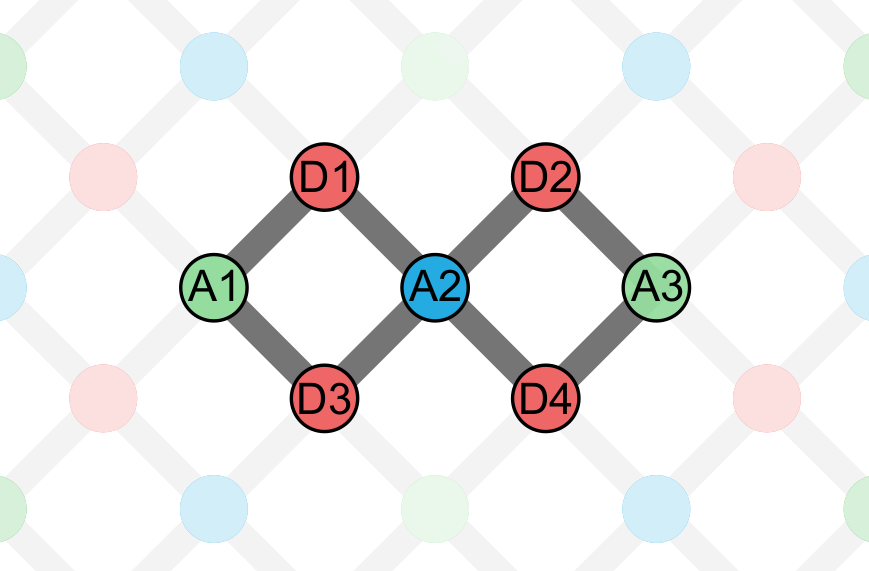
\includegraphics[width=0.4\textwidth]{images/seven_qbit_code.png}
  \caption{A seven qubit surface code, with four red data qubits, one blue
    X-type ancilla and 2 Z-type ancilla qubits. This is the smallest viable
    instance of the surface code.}
  \label{fig:seven_qbit_code}
\end{figure}

Remarkably, despite an inability to explicitly correct for detected errors,
Andersen \textit{et al.}, by measuring ancillas for errors, can ensure a longer
logical qubit lifetime than any physical qubit lifetime for the data qubits
which comprise the logical qubit. By checking repeatedly that no stabilizer
measurement has fired, they show that the decay of the expectation values
$\langle Z_L \rangle$ and $\langle X_L \rangle$ both exceed equivalent
expectation values for the best physical data qubit. Repeated stabilizer
measurement outcomes that signal no error whatsoever are possible here are a
testament to the precision with which superconducting qubits can be initialized,
manipulated and measured. As further research realizes qubits with error rates
further and further below the error threshold for reliable error correction,
larger codes and better stabilizer measurement can make large-scale,
fault-tolerant computation possible. Versluis \textit{et al.} have proposed a
scheme for scalable QEC using transmon superconducting qubits that focuses on
developing an eight-qubit unit cell that can be used to tile together a full
surface code \cite{Versluis_2017}.

Implementations of the surface code are not only limited to superconducting
qubits, either. Recent proposals, such as that of Hill \textit{et al.} , to
implement the surface code in silicon quantum dots promise to drastically reduce
the overhead per qubit by exploiting the uniformity between phosphorus donor
nuclear spin qubits \cite{silicon_surface_code}. Their proposal addresses the
requirement for repeated stabilizer measurement by implementing shared control
over all the qubits, resulting in a control architecture capable of executing
the full sequence of CNOT gates for all ancilla qubits in just four steps. The
number of steps required is independent of qubit number, which makes this
approach eminently scalable. Though the results presented by Hill \textit{et
  al.} are simulations, the authors stress that all the key requirements for
implementing this scheme in a physical system have already been demonstrated.

%%% Local Variables:
%%% mode: latex
%%% TeX-master: "QEC_paper"
%%% End:
